\begin{figure}%[!htp]
	\centering
	\setlength{\imagewidth}{120mm}%
	\setlength{\imageheight}{0.625\imagewidth}%
	\DTLsetseparator{,}%
	\DTLloaddb[noheader,keys={x,y}]{dbsurfpoint}{figures/data/EdS_propre_carreau/surface_point.dat}%
	\DTLloaddb[noheader,keys={x,y}]{dbsurfvectors}{figures/data/EdS_propre_carreau/surface_vectors.dat}%
	\DTLloaddb[noheader,keys={x,y}]{dbEdSpoints}{figures/data/EdS_propre_carreau/envelope_points.dat}%
	\DTLloaddb[noheader,keys={x,y}]{dbEdSnormals}{figures/data/EdS_propre_carreau/envelope_normals.dat}%
	\begin{tikzpicture}[
		x = \imagewidth,
		y = \imageheight,
		point/.style = {circle, scale=0.27, fill=black},
		vector/.style = {-latex', thick},
		label/.style = {inner sep=2pt},
		txt/.style = {font=\small}
	]
		\node[anchor=south west, inner sep=0] at (0,0) {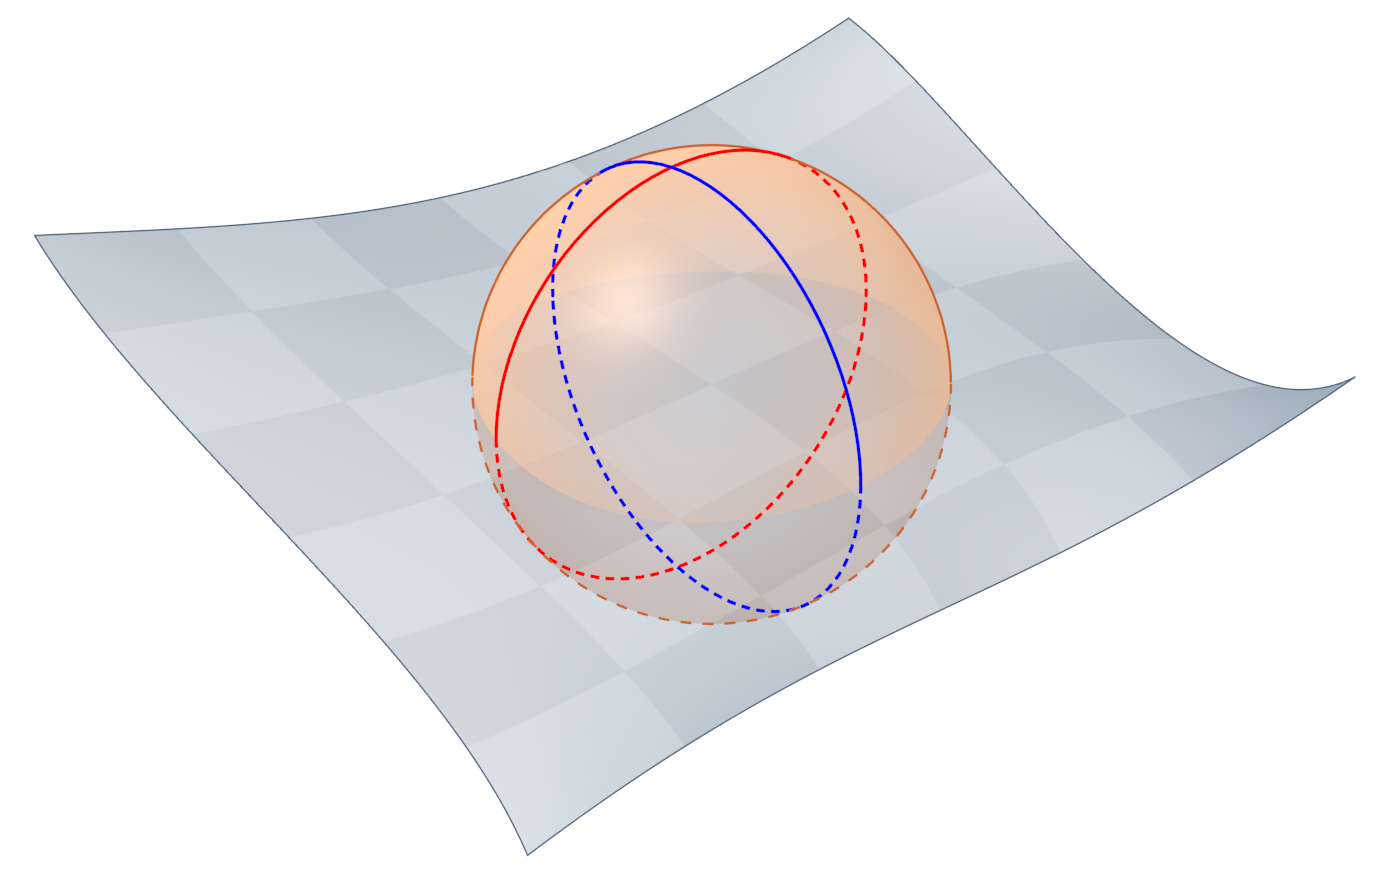
\includegraphics[width=\imagewidth]{figures/images/EdS_propre_carreau/EdS_propre_carreau.png}};
		%\drawGrid{10}{10}{black, thin, dotted}
		\DTLassign{dbsurfpoint}{1}{\spx=x, \spy=y}
		\coordinate (s) at (\spx, \spy);
		%
		\DTLassign{dbEdSpoints}{1}{\eppx=x, \eppy=y}
		\DTLassign{dbEdSpoints}{2}{\empx=x, \empy=y}
		\coordinate (ep) at (\eppx, \eppy);
		\coordinate (em) at (\empx, \empy);
		\node [anchor=north, txt, xshift=0pt, label] at (ep) {$\eos^+$};
		\node [anchor=south, txt, xshift=3pt, yshift=2pt, label] at (em) {$\eos^-$};
		%
		\DTLassign{dbsurfvectors}{1}{\sux=x, \suy=y}
		\coordinate (su) at (\sux, \suy);
		\draw [vector, red] (s) -- (su) node [below, xshift=-1pt, label, txt] {$\bsu$};
		%
		\DTLassign{dbsurfvectors}{2}{\svx=x, \svy=y}
		\coordinate (sv) at (\svx, \svy);
		\draw [vector, blue] (s) -- (sv) node [above, xshift=-4pt, label, txt] {$\bsv$};
		%
		\DTLassign{dbsurfvectors}{3}{\snx=x, \sny=y}
		\coordinate (sn) at (\snx, \sny);
		\draw [vector] (s) -- (sn) node [right, label, txt, black] {$\unv$};
		%
		\DTLassign{dbEdSnormals}{1}{\epnx=x, \epny=y}
		\coordinate (epn) at (\epnx, \epny);
		\node [anchor=west, label, txt, xshift=0pt] at (epn) {$\unv_{\envelope}^+$};
		\draw [dotted, thick, shorten >= 14pt] (s) -- (ep);
		\draw [vector] (ep) -- (epn);
		%
		\DTLassign{dbEdSnormals}{2}{\emnx=x, \emny=y}
		\coordinate (emn) at (\emnx, \emny);
		\node [anchor=west, label, txt, xshift=0pt] at (emn) {$\unv_{\envelope}^+$};
		\draw [dotted, thick, shorten <= 0pt, shorten >= 14pt] (s) -- (em);
		\draw [vector] (em) -- (emn);
		%
		\node [point] at (s) {};
		\node [point] at (ep) {};
		\node [point] at (em) {};
		%
		\node [anchor=east, txt, inner sep=2pt] at (s) {$\bs(u,v)$};
		\definecolor{colorSurfLabel}{rgb}{0.330, 0.413, 0.500}
		\node [txt, label, colorSurfLabel] at (0.1,0.68) {$\Sigma_i$};
	\end{tikzpicture}
	\DTLgdeletedb{dbsurfpoint}%
	\DTLgdeletedb{dbsurfvectors}%
	\DTLgdeletedb{dbEdSpoints}%
	\DTLgdeletedb{dbEdSnormals}%
	\caption{Paramétrisation de l'EdS propre d'un carreau paramétrique.}
	\label{fig:EdS_propre_carreau}
\end{figure}